% Engineering-method manuscript. Formula source: docs/formula.md; empirical source: docs/euroc_final_results.md.
\documentclass[a4paper,runningheads,twocolumn]{llncs}
% Two-column reading layout for the English draft only.
\usepackage[a4paper,margin=20mm,headheight=14pt,headsep=7mm]{geometry}
\usepackage{adjustbox}
\setlength{\columnsep}{7mm}
\setlength{\dbltextfloatsep}{12pt plus 2pt minus 2pt}
\setlength{\textfloatsep}{10pt plus 2pt minus 2pt}
\renewcommand{\dbltopfraction}{0.9}
\renewcommand{\textfraction}{0.08}
\renewcommand{\floatpagefraction}{0.75}
\renewcommand{\dblfloatpagefraction}{0.75}
\setcounter{dbltopnumber}{3}
\usepackage[T1]{fontenc}
\usepackage{lmodern}
\usepackage{amsmath,amssymb,bm}
\usepackage{graphicx,booktabs}
\usepackage{tikz}
\usetikzlibrary{arrows.meta,positioning}
\usepackage{xurl}
\usepackage[hidelinks]{hyperref}
\hypersetup{pdftitle={Robust Visual-Inertial Odometry with Linear Time-Varying Observer-Aided Constraints},pdfauthor={liuhe},pdfsubject={Engineering method and empirical evaluation},pdfkeywords={VIO, LTV Observer, ESKF, MSCKF}}
\newcommand{\R}{\mathbb{R}}
\newcommand{\sk}[1]{[#1]_{\times}}
\newcommand{\diag}{\operatorname{diag}}
\newcommand{\tr}{\operatorname{tr}}
\newcommand{\Exp}{\operatorname{Exp}}
\newcommand{\norm}[1]{\left\lVert #1\right\rVert}
\newcommand{\placeholder}[1]{\par\smallskip\noindent\textit{[Figure placeholder: #1]}\par\smallskip}
\emergencystretch=1em

\begin{document}
\title{Robust Visual-Inertial Odometry with Linear Time-Varying Observer-Aided Constraints}
\titlerunning{LTV Observer-Aided Visual-Inertial Odometry}
\author{liuhe}
\authorrunning{liuhe}
\institute{Huazhong University of Science and Technology, Wuhan, China\\
\email{liuhe2024@hust.edu.cn}}
\twocolumn[
\begin{@twocolumnfalse}
\maketitle

\begin{abstract}
Body-frame linear time-varying (LTV) observers offer an alternative representation of visual-inertial motion, but using their outputs inside an existing filter requires explicit treatment of coordinates, timing, and fusion strength. This paper presents an engineering integration of an LTV observer with OpenVINS. We retain the continuous model as the design background and specify a discrete implementation for asynchronous IMU propagation, bearing correction, and bounded landmark management. Observer gravity, velocity, and landmark estimates are converted into error-state auxiliary measurements with first-estimate Jacobians. Accepted auxiliary blocks are combined with MSCKF visual residuals at one main-filter prior. Branch checks and a covariance-relative landmark budget control fusion under an explicit shared-observation correlation approximation. An archived five-mode EuRoC evaluation compares accuracy, local errors, actual auxiliary use, and serial runtime. Velocity and full fusion reduce position ATE on all four evaluated Machine Hall sequences, with mean relative reductions of 7.410\% and 7.578\%, while Vicon changes remain small. Substantial measured overhead and the tuned evaluation protocol bound these findings. The contribution is the observer-to-filter integration and its empirical assessment.
\keywords{Visual-inertial odometry \and Linear time-varying observer \and Error-state Kalman filter \and Auxiliary constraints}
\end{abstract}
\vspace{6mm}
\end{@twocolumnfalse}
]

\section{Introduction}
Reliable motion estimation is essential for autonomous robots operating without an external positioning system. Cameras provide geometric constraints, while an inertial measurement unit (IMU) supplies high-rate rotational and translational motion information. Their complementary characteristics motivate visual-inertial odometry (VIO). Nevertheless, motion estimation remains sensitive to the available feature geometry, motion excitation, inertial bias, and the relative strength of the fused constraints.

Filter-based VIO maintains a motion state and its uncertainty while using image observations to correct inertial propagation. The stereo multi-state constraint Kalman filter (S-MSCKF) uses historical camera poses to obtain visual constraints without retaining every feature as a persistent filter state~\cite{sun2018}. OpenVINS provides a modular implementation of this approach, including first-estimate Jacobians (FEJ), calibrated sensor models, and flexible state management~\cite{geneva2020}. These systems are suitable platforms for studying auxiliary measurements because new residual blocks can be related directly to existing error-state variables.

A complementary perspective is to formulate motion quantities in the moving body frame. Wang and Tayebi~\cite{wang2024} introduce an LTV observer that estimates body-frame landmark positions, velocity, and gravity from inertial inputs and bearing observations. This representation avoids including attitude explicitly in the corresponding linear state. It suggests an opportunity to use these estimated quantities as auxiliary constraints within an established VIO estimator, while retaining the latter's inertial bias estimation and multi-view visual update.

The engineering question is how to reuse these body-frame estimates within a native VIO filter and establish when the resulting constraints are useful. The observer shares IMU, bearings, geometric seeds, and bias estimates with the main filter; its outputs are therefore correlated auxiliary estimates. Their value must be assessed empirically, with fusion strength and computational cost reported. Translating these outputs into usable error-state constraints also requires consistent geometry and timing. A gravity vector should constrain its direction without adding an artificial magnitude measurement. A body-frame velocity observation depends jointly on attitude and world-frame velocity. A landmark estimate requires a consistent temporal anchor and coordinate transformation. In addition, measurements computed at one prior must not be submitted after that prior has changed. These considerations motivate the unified fusion interface developed here.

We study three branches, denoted G, V, and L, and their full combination GVL. The implementation uses the existing stereo frontend and an LTV side estimator; it does not introduce an additional sensor or an external map. An archived evaluation on EuRoC~\cite{burri2016} examines the accuracy benefit and computational cost of the observer-aided fusion scheme. The remainder of the paper presents the theoretical preliminaries, the fusion method, the experiments, and the conclusions. The main contributions are:
\begin{enumerate}
\item An observer-to-filter measurement formulation for body-frame gravity, velocity, and temporally anchored landmarks, with Jacobians and snapshot timing matched to the native VIO state convention.
\item A common-prior integration interface that combines accepted auxiliary and native visual blocks, with branch gates and a landmark fusion budget under an explicit shared-observation correlation approximation.
\item An empirical assessment using archived five-mode comparisons, reporting trajectory and local errors, actual auxiliary use, failures and exclusions, and serial computational overhead, with the limits of tuned comparisons identified.
\end{enumerate}

\section{Theoretical Preliminaries}
\subsection{Frames, Inertial Inputs, and Bearing Geometry}
Let $\{W\}$, $\{B\}$, and $\{C\}$ denote the world, IMU body, and camera frames. We use $R\in SO(3)$ to map world-frame vectors into the body frame. Position $p$ and velocity $v$ are expressed in $\{W\}$, and $g_W=[0,0,-g]^\top$ is physical gravity. For $u\in\R^3$, $\sk{u}$ satisfies $\sk{u}w=u\times w$. Hats denote estimates and superscripts $-$ and $+$ denote prior and posterior quantities.

With calibrated, bias-corrected IMU inputs $\omega$ and $a$, the nominal kinematics are
\begin{equation}
 \dot R=-\sk{\omega}R,\qquad
 \dot p=v,\qquad
 \dot v=R^\top a+g_W .
 \label{eq:kinematics}
\end{equation}
Here $a$ is specific force, not acceleration with gravity already removed. Bias correction is applied once, using the current VIO bias estimates and the fixed sensor calibration.

Let $R_{BC}$ map camera vectors into the body frame, and let $p_{BC}$ be the camera center expressed in the body frame. For a static world point $P_i$, define its body-frame position
\begin{equation}
 \ell_i=R(P_i-p),\qquad
 P_i^C=R_{BC}^{\top}(\ell_i-p_{BC}).
 \label{eq:pointframes}
\end{equation}
A calibrated image coordinate yields the unit bearing
\begin{equation}
 b_i=\frac{[u_i^{n},v_i^{n},1]^\top}
 {\norm{[u_i^{n},v_i^{n},1]^\top}},\qquad d_i=R_{BC}b_i .
\end{equation}
The projection $\Pi_i=I_3-d_id_i^\top$ removes the unknown depth and gives the linear relation
\begin{equation}
 y_i=\Pi_i p_{BC}=\Pi_i\ell_i .
 \label{eq:bearing}
\end{equation}
All camera extrinsics and timestamps are transformed into the same body-frame convention before constructing observer inputs.
\placeholder{World, IMU body, and camera frames; camera offset $p_{BC}$, unit bearing $b_i$, and body-frame landmark $\ell_i$.}

\subsection{Body-Frame LTV Observer}
Following the body-frame formulation in~\cite{wang2024}, introduce $v_B=Rv$ and $\eta=Rg_W$. Their dynamics, together with those of the static landmarks, are
\begin{equation}
 \begin{aligned}
 \dot\ell_i&=-\sk{\omega}\ell_i-v_B,\\
 \dot v_B&=-\sk{\omega}v_B+\eta+a,\\
 \dot\eta&=-\sk{\omega}\eta .
 \end{aligned}
 \label{eq:ltvdynamics}
\end{equation}
For a fixed set of $N$ static landmarks in the continuous model, let
\begin{equation}
 \begin{gathered}
 z=[\ell_1^\top,\ldots,\ell_N^\top,v_B^\top,\eta^\top]^\top,\\
 \dot z=Az+Ba,\quad y=Cz .
 \end{gathered}
 \label{eq:ltvstate}
\end{equation}
Writing $\Omega_N=\diag(\sk{\omega},\ldots,\sk{\omega})$ and
$\Gamma=\bm{1}_N\otimes I_3$, the matrices are
\begin{equation}
 \begin{gathered}
 A=\begin{bmatrix}
 -\Omega_N&-\Gamma&0\\
 0&-\sk{\omega}&I_3\\
 0&0&-\sk{\omega}
 \end{bmatrix},\\
 B=\begin{bmatrix}0\\I_3\\0\end{bmatrix},\quad
 C=\begin{bmatrix}\diag(\Pi_1,\ldots,\Pi_N)&0&0\end{bmatrix}.
 \end{gathered}
 \label{eq:ltvmatrices}
\end{equation}
Here $z\in\R^{n_o}$ with $n_o=3N+6$, $A\in\R^{n_o\times n_o}$, $B\in\R^{n_o\times3}$, and $C\in\R^{3N\times n_o}$. The continuous observer and its design matrix $P_o$ satisfy
\begin{align}
 \dot{\hat z}&=A\hat z+Ba+K_L(y-C\hat z),\label{eq:observer}\\
 K_L&=P_oC^\top Q_L, \notag\\
 \dot P_o&=AP_o+P_oA^\top-P_oC^\top Q_LCP_o+V_L .
 \label{eq:riccati}
\end{align}
The uniformly positive-definite design matrices $Q_L$ and $V_L$ weight the bearing correction and the Riccati regularization, respectively; $P_o$ sets the observer gain. These design objects are distinct from the main EKF covariance and the auxiliary measurement noise introduced below.

Wang and Tayebi~\cite{wang2024} establish exponential convergence for their continuous LTV observer under persistent excitation of the world-frame bearing directions, the associated uniform observability, bounded and uniformly continuous angular velocity, and the stated regularity and positivity assumptions on the design matrices and initial $P_o$. We cite that result as the design motivation for the original system. The discrete implementation with changing feature sets and filter-derived inputs is specified separately, without asserting that it inherits the original convergence guarantee. The separate nonlinear pose observer in~\cite{wang2024} is not used here.

\subsection{Error-State Filtering and MSCKF Visual Constraints}
The VIO state contains the current inertial state and historical IMU pose clones:
\begin{equation}
 \begin{aligned}
 x&=(R,p,v,b_g,b_a,x_{c_1},\ldots,x_{c_M}),\\
 \delta x_I&=[\delta\theta^\top,\delta p^\top,\delta v^\top,
              \delta b_g^\top,\delta b_a^\top]^\top .
 \end{aligned}
\end{equation}
Our attitude error is defined by
\begin{equation}
 R_{\mathrm{true}}=\Exp(-\sk{\delta\theta})\hat R
       \simeq (I_3-\sk{\delta\theta})\hat R .
 \label{eq:attitudeerror}
\end{equation}
Vector errors are additive. The corresponding linearized inertial model is
$\delta\dot x_I=F\delta x_I+Gn_I$. Discretization gives the transition $\Phi_k$ and integrated process noise $Q_k$, so
\begin{equation}
 P_{I,k+1}^-=\Phi_kP_{I,k}^+\Phi_k^\top+Q_k .
 \label{eq:covprop}
\end{equation}
Cross-covariances with the clones are propagated consistently. At an image event, the current pose is cloned through its augmentation Jacobian. This retains the correlations needed for multi-view constraints~\cite{sun2018,geneva2020}.

For a feature observed at several poses, linearization yields
\begin{equation}
 r_f=H_x\delta x+H_f\delta P_f+n_f .
\end{equation}
With isotropic pixel noise $\mathcal R_f=\sigma_{\mathrm{pix}}^2I$, an orthonormal left-nullspace basis $U$ with $U^\top H_f=0$ and $U^\top U=I$ eliminates the feature error:
\begin{equation}
 r_{\mathrm{vis}}=U^\top r_f,\qquad
 H_{\mathrm{vis}}=U^\top H_x,\qquad
 \mathcal R_{\mathrm{vis}}=U^\top\mathcal R_fU .
 \label{eq:msckf}
\end{equation}
Accepted feature blocks are stacked and compressed before the EKF update. FEJ evaluates the required Jacobians at stored first estimates, while residuals use the current state. In our experiments, calibration is fixed and native SLAM landmarks are disabled. Features are still tracked and triangulated for MSCKF constraints.

\section{LTV Observer-Aided ESKF Fusion}
Based on the continuous-time model above, we construct a discrete observer for asynchronous IMU and camera inputs and convert its outputs into auxiliary constraints for the main filter.

\subsection{Discrete Implementation of the LTV Observer}
\label{sec:discrete}
\paragraph{IMU propagation.}
The observer is advanced to camera time in the IMU clock, $t_I=t_C+\delta t_{C\to I}$. Bracketed samples are calibrated and bias-corrected once, using biases saved before main-state propagation. For each positive interval $\Delta t_k$, the corrected endpoint samples are averaged to obtain $\bar a_k,\bar\omega_k$. The first-order state and design propagation is
\begin{equation}
 \begin{aligned}
 F_{o,k}&=I_{n_o}+\Delta t_k A(\bar\omega_k),\\
 \hat z_{k+1}^-&=F_{o,k}\hat z_k+\Delta t_k B\bar a_k,\\
 P_{o,k+1}^-&=F_{o,k}P_{o,k}F_{o,k}^\top+\Delta t_kV_o.
 \end{aligned}
 \label{eq:discreteprop}
\end{equation}
Here $V_o=\diag(\nu_\ell I_{3N},\nu_vI_3,\nu_\eta I_3)$ weights the landmark, velocity, and gravity design blocks. $P_o$ is symmetrized after propagation and correction; invalid times, nonfinite inputs, or failed numerical checks invalidate the observer event.

\paragraph{Camera correction.}
After feature synchronization, the current camera-0 bearings select $3M_c$ observed rows from the projection model~\eqref{eq:bearing}, giving $y_c,C_c$. For elapsed camera-event time $\Delta t_c>0$, the correction is
\begin{equation}
 \begin{aligned}
 \mathcal R_o&=(q_\ell\Delta t_c)^{-1}I_{3M_c},\\
 K_o&=P_{o,c}^-C_c^\top
       (C_cP_{o,c}^-C_c^\top+\mathcal R_o)^{-1},\\
 \hat z_c^+&=\hat z_c^-+K_o(y_c-C_c\hat z_c^-),\\
 P_{o,c}^+&=J_oP_{o,c}^-J_o^\top+K_o\mathcal R_oK_o^\top,
 \end{aligned}
 \label{eq:discretecorrect}
\end{equation}
with $J_o=I_{n_o}-K_oC_c$. LLT solves compute the gain, and the Joseph form is used for the design matrix. Correction is skipped at the first camera event or when $M_c=0$. This event-based recursion is the numerical realization of the continuous design; $P_o$ and $\mathcal R_o$ remain separate from the main covariance and auxiliary noise.

\paragraph{Features and history.}
A bounded pool retains at most 30 landmarks, initialized from stereo geometry or temporal bearings with live main-filter poses. Accepted births receive their body-frame seed and an isotropic initial design block with zero cross-blocks; retained states preserve all mutual cross-blocks, and retirement deletes the corresponding rows and columns. Seed uncertainty is used for admission rather than assigned to $P_o$. Feature identity and epoch checks prevent stale associations. For L, the current point is captured after IMU propagation and before feature synchronization and bearing correction. Post-camera points are saved as future anchors before the main EKF update, and anchors without live clones are removed. G/V use the current post-camera outputs. Full initialization checks and configuration details are recorded in the implementation documentation.

\subsection{Common-Prior Fusion Interface}
Figure~\ref{fig:framework} shows the integration. The main filter supplies bias estimates, geometric seed poses, the current prior, and live clones. All enabled modes run the same landmark/velocity/gravity observer; the mode controls which outputs become additional main-filter rows.

\begin{figure*}[t]
\centering
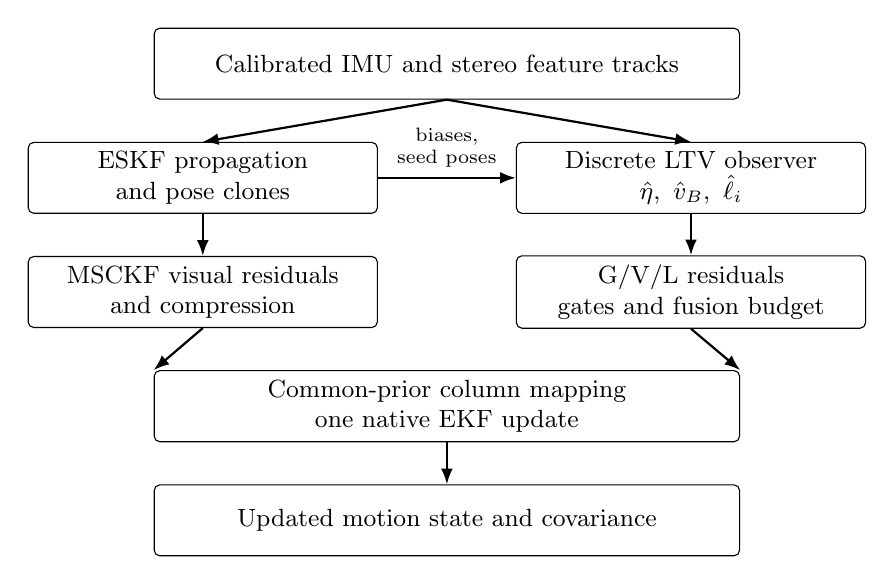
\begin{tikzpicture}[font=\small,
 box/.style={draw,rounded corners=2pt,align=center,minimum height=9mm,text width=42mm},
 flow/.style={-{Latex[length=2mm]},thick}]
\node[box,text width=72mm] (input) at (0,0) {Calibrated IMU and stereo feature tracks};
\node[box] (vio) at (-3.1,-1.45) {ESKF propagation\\and pose clones};
\node[box] (ltv) at (3.1,-1.45) {Discrete LTV observer\\$\hat\eta,\ \hat v_B,\ \hat\ell_i$};
\node[box] (vis) at (-3.1,-2.9) {MSCKF visual residuals\\and compression};
\node[box] (aux) at (3.1,-2.9) {G/V/L residuals\\gates and fusion budget};
\node[box,text width=72mm] (joint) at (0,-4.35) {Common-prior column mapping\\one native EKF update};
\node[box,text width=72mm] (out) at (0,-5.8) {Updated motion state and covariance};
\draw[flow] (input.south) -- (vio.north);
\draw[flow] (input.south) -- (ltv.north);
\draw[flow] (vio.east) -- node[above,font=\scriptsize,align=center] {biases,\\seed poses} (ltv.west);
\draw[flow] (vio) -- (vis);
\draw[flow] (ltv) -- (aux);
\draw[flow] (vis.south) -- (joint.north west);
\draw[flow] (aux.south) -- (joint.north east);
\draw[flow] (joint) -- (out);
\end{tikzpicture}
\caption{Observer-aided VIO with shared sensor inputs and main-state feedback. Landmark candidates for L are captured before current bearing correction; G/V use post-correction estimates. Auxiliary branches may be rejected separately.}
\label{fig:framework}
\end{figure*}

Each auxiliary block contains a residual $r_j$, a local Jacobian $H_j$, noise $\mathcal R_j$, and an ordered list of native state variables. The host checks camera/IMU time agreement, variable ownership, dimensions, and finite values. State identity, epoch, and sequence number prevent repeated or stale auxiliary-event submission. Blocks are built and merged synchronously against the unchanged main prior; the auxiliary model itself does not modify the main state.

For all branches, $r=z_{\mathrm{aux}}-h(\hat x)\simeq H\delta x+n$, so $H$ differentiates the prediction. Superscript $f$ denotes FEJ values when enabled and current values otherwise. Residuals always use the current prior, and observer outputs are held fixed when forming the main-state Jacobians.

\subsection{Gravity Direction Constraint}
Let $\gamma=g_W/\norm{g_W}$, $u_G=\hat\eta/\norm{\hat\eta}$, and $d^f=R^f\gamma$. To construct the tangent basis, choose $e_h$ with $h=\arg\min_h|d_h^f|$ and set
\begin{equation}
 \begin{gathered}
 t_1=\frac{e_h-d^f(d^{f\top}e_h)}{\norm{e_h-d^f(d^{f\top}e_h)}},\\
 t_2=d^f\times t_1,\qquad T=[t_1\ t_2].
 \end{gathered}
 \label{eq:gravitybasis}
\end{equation}
Then $T^\top T=I_2$ and $T^\top d^f=0$. With local columns $[\delta\theta_t,\delta v_t]$ and $T$ fixed during linearization,
\begin{equation}
 \begin{aligned}
 r_G&=T^\top(u_G-\hat R\gamma),\\
 H_G&=[T^\top\sk{R^f\gamma}\quad0_{2\times3}],\\
 \mathcal R_G&=\sigma_G^2I_2,\qquad
 \sigma_G=\frac{10\pi/180}{\sqrt{\alpha_G}}.
 \end{aligned}
 \label{eq:gravity}
\end{equation}
This gives two direction rows and no gravity-magnitude measurement. The residual is dimensionless; the angular noise scale is a small-error approximation. G directly constrains attitude relative to gravity, without supplying an independent global position or heading reference.

\subsection{Body-Frame Velocity Constraint}
With the same six local columns as G,
\begin{equation}
 \begin{aligned}
 r_V&=\hat v_B-\hat R\hat v,\\
 H_V&=[\sk{R^fv^f}\quad R^f],\\
 \mathcal R_V&=\sigma_V^2I_3,\qquad
 \sigma_V=\frac{1~\mathrm{m/s}}{\sqrt{\alpha_V}}.
 \end{aligned}
 \label{eq:velocity}
\end{equation}
The two Jacobian blocks follow from the JPL left attitude perturbation and additive world-frame velocity error. Using both blocks is necessary because attitude changes the predicted body-frame velocity. Main-state cross-covariances can also transmit the update to position and biases. The observer velocity design block is not substituted for $\mathcal R_V$.

\subsection{Temporally Anchored Landmark Constraint}
For a historical post-camera snapshot $\hat\ell_{i,a}^+$ at a live pose clone and a current pre-camera estimate $\hat\ell_{i,t}^-$, define
\begin{equation}
 \begin{aligned}
 h_{L,i}(x)&=R_t\big(R_a^\top\hat\ell_{i,a}^++p_a-p_t\big),\\
 r_{L,i}&=\hat\ell_{i,t}^--h_{L,i}(\hat x).
 \end{aligned}
 \label{eq:landmark}
\end{equation}
The past landmark and anchor pose jointly construct a world point; it is not an independent known map point. For local columns $[\delta\theta_t,\delta p_t,\delta\theta_a,\delta p_a]$, the prediction Jacobian is
\begin{equation}
 \begin{gathered}
 H_{L,i}=[H_{\theta_t}\ H_{p_t}\ H_{\theta_a}\ H_{p_a}],\\
 H_{\theta_t}=\sk{h_{L,i}^f},\qquad H_{p_t}=-R_t^f,\\
 H_{\theta_a}=-R_t^f(R_a^f)^\top\sk{\hat\ell_{i,a}^+},\qquad
 H_{p_a}=R_t^f,\\
 h_{L,i}^f=R_t^f\big((R_a^f)^\top\hat\ell_{i,a}^++p_a^f-p_t^f\big).
 \end{gathered}
 \label{eq:landmarkH}
\end{equation}
Residuals use current poses; only the pose Jacobians use FEJ. Historical landmark values do not acquire separate FEJ states. The direct measurement variables are current attitude and position plus the whole anchor pose clone; observer points are not written into native SLAM states.

Candidates require maturity and the velocity-readiness flag available before the current camera correction, even in L-only mode. This flag can differ from the post-correction readiness used by G/V. For span $\tau_i=t-t_a$, the checks include
\begin{equation}
 \begin{gathered}
 0.20~\mathrm{s}\leq\tau_i\leq0.55~\mathrm{s},\\
 \frac{\norm{\hat\ell_{i,t}^--h_{L,i}(\hat x)}}
 {\max(\norm{h_{L,i}(\hat x)},0.1~\mathrm{m})}\leq0.02.
 \end{gathered}
 \label{eq:lvalid}
\end{equation}
The span test permits $10^{-6}$ s boundary tolerance. Both points transformed into current camera 0 must have finite coordinates, range at least 0.1 m, and positive optical depth, with valid feature association. The first chronological anchor with a live clone is examined; a failed gate does not cause a search through later anchors. Candidates are sorted by feature ID, and at most $m_{\max}=2$ passing points are selected.

Range, age, and the main marginal covariance determine the effective noise:
\begin{equation}
 \begin{aligned}
 s_{i,0}^2&=\big(\sigma_{L,0}+0.02\norm{\hat\ell_{i,t}^-}\big)^2
       \left(1+\frac{\tau_i}{0.55~\mathrm{s}}\right),\\
 q_i&=\tr(H_{L,i}P_i^-H_{L,i}^{\top}),\\
 s_i^2&=\max\left(s_{i,0}^2,\frac{q_i}{\beta_L/m_{\max}}\right),\\
 \mathcal R_{L,i}&=s_i^2I_3,\qquad
 \sigma_{L,0}=\frac{0.5~\mathrm m}{\sqrt{\alpha_L}},\quad
 \beta_L=0.01\alpha_L.
 \end{aligned}
 \label{eq:lbudget}
\end{equation}
$P_i^-$ retains all cross-blocks of the current and anchor poses. The noise is enlarged before computing the gain, giving $q_i/s_i^2\leq\beta_L/m_{\max}$. The cap is allocated using the configured maximum count, without reallocating unused shares. It limits the normalized predicted variance under the adopted noise model, not the true information in correlated observations. No resulting state correction is clipped, and L has no separate NIS-threshold or Huber rejection step.

\subsection{Readiness, Gates, and Fusion Strength}
A frame must have valid time/epoch information and pass warmup before auxiliary construction. By default, 20 consecutive image events with at least 15 observed features establish frame warmup. Branch readiness additionally requires at least 15 mature visible features, 20 actual camera corrections, a physically plausible gravity norm, and healthy prediction/correction diagnostics. For camera-0 predicted rays, the diagnostic angle is the arccosine of their normalized dot product with the current bearing. Its P95 limit is 0.02 rad. Correction rates are
\begin{equation}
 c_v=\frac{\norm{\hat v_B^+-\hat v_B^-}}{\Delta t_c},\qquad
 c_\eta=\frac{\norm{\hat\eta^+-\hat\eta^-}}{\Delta t_c}.
 \label{eq:healthrates}
\end{equation}
The health gravity interval is $[8,11.5]$ m/s$^2$. G requires $c_\eta\leq1$ m/s$^3$; V also requires $c_v\leq0.5$ m/s$^2$. Each branch needs 20 confirming frames. Once confirmed, the default soft grace allows at most two consecutive soft failures within 0.10 s of the last strictly good event, provided hard validity holds and angle/rate diagnostics remain within twice their strict limits.

G also checks $\norm{\hat\eta}\in[7,12]$ m/s$^2$ and the two direction conditions
\begin{equation}
 \begin{gathered}
 \arccos\!\left(\operatorname{clamp}(u_G^\top\hat R\gamma,-1,1)\right)
      \leq30\pi/180,\\
 u_G^\top R^f\gamma>0.
 \end{gathered}
 \label{eq:gravitygate}
\end{equation}
The latter fixes the accepted hemisphere relative to the tangent-plane linearization direction. V requires a finite valid velocity output. L uses the pre-correction eligibility above and still requires the current frame to pass warmup.

Let $E_j$ select a block's local variables from the full main error state and $P_j^-=E_jP^-E_j^\top$. G/V NIS gating uses
\begin{equation}
 S_j=H_jP_j^-H_j^\top+\mathcal R_j,\qquad
 \nu_j=r_j^\top S_j^{-1}r_j\leq\eta_j.
 \label{eq:nis}
\end{equation}
Default thresholds are $\eta_G=9.21034$ and $\eta_V=11.34487$, corresponding to 99\% chi-square thresholds for two and three rows. LLT solves evaluate NIS. Even with threshold rejection disabled, G/V require valid nonnegative NIS, positive-definite noise, and a successful finite innovation factorization. L and the final joint block undergo structural and numerical checks, but their recorded NIS has no separate threshold rejection.

Optional quality gating checks at least 25 observed features and innovation norm divided by $\sqrt{\max(1,3M_c)}$ at most 0.03 m. G additionally checks gravity-magnitude error at most 0.5 m/s$^2$, and V checks velocity disagreement at most 0.5 m/s. Optional Huber weighting is applied to G/V after their original-noise NIS gate: for $\mathcal R_j=L_jL_j^\top$, set $s_j=\norm{L_j^{-1}r_j}$ and multiply $\mathcal R_j$ by $\max(1,s_j/\delta_H)$, with default $\delta_H=2$. This uses noise whitening rather than innovation whitening, and no nonlinear iteration is performed. Quality gating and Huber weighting are disabled by default. Enabled weights must be finite and positive; increasing a weight changes the noise and therefore the computed gain, without multiplying the state correction directly.

\subsection{Joint Native EKF Update and Correlation Approximation}
Using $\bar H_j=H_jE_j$ maps all blocks into a common full-state column layout. After native visual compression and auxiliary selection, form
\begin{equation}
 \begin{gathered}
 r=[r_{\mathrm{vis}}^\top\ r_G^\top\ r_V^\top\ r_L^\top]^\top,\\
 \bar H=[\bar H_{\mathrm{vis}}^\top\ \bar H_G^\top\
          \bar H_V^\top\ \bar H_L^\top]^\top,\\
 \mathcal R_{\mathrm{eff}}=\diag(\mathcal R_{\mathrm{vis}},
                  \mathcal R_G,\mathcal R_V,\mathcal R_L).
 \end{gathered}
 \label{eq:joint}
\end{equation}
Rejected or disabled blocks contribute no rows. G and V supply two and three rows, respectively, and each selected L point supplies three; the default auxiliary maximum is eleven rows. The implementation stores only the union of native variable columns and uses its marginal covariance, while retaining the full-state cross-covariances needed for the gain. A shared variable appears only once; incompatible overlapping variable ranges are rejected.

All accepted blocks use one main prior. In full-state notation, the native update is
\begin{equation}
 \begin{aligned}
 S&=\bar HP^-\bar H^\top+\mathcal R_{\mathrm{eff}},\\
 K&=P^-\bar H^\top S^{-1},\qquad\delta\hat x=Kr,\\
 x^+&=x^-\boxplus\delta\hat x,\\
 P^+&=P^--K(P^-\bar H^\top)^\top.
 \end{aligned}
 \label{eq:ekf}
\end{equation}
The covariance expression equals $P^--KSK^\top$ in exact arithmetic. Native code uses the upper triangle and restores symmetry; this main covariance update is not the observer Joseph update. Cholesky solves construct the innovation inverse action; the native routine solves against an identity matrix when computing its gain. Mean injection uses additive vector corrections and a normalized small-angle JPL quaternion left update consistent with~\eqref{eq:attitudeerror}; ordinary mean updates leave FEJ values unchanged.

The block-diagonal effective noise ignores cross-correlations among visual and auxiliary errors and between those errors and the main prior. The common-prior update, gates, and noise inflation organize and limit this approximation; they do not establish statistical independence or full-filter consistency. Observer $P_o$, main covariance $P$, and auxiliary noise $\mathcal R_j$ have separate roles throughout the method. The proposed contribution is a controlled integration with empirical evaluation, rather than a new convergence guarantee for the coupled system.

The per-image procedure is:
\begin{enumerate}
\item Save the main bias estimates, propagate and clone the main state, and advance the observer to the corresponding IMU time.
\item Capture pre-correction L candidates; prepare feature births/retirements, synchronize the observer layout, and apply bearing correction.
\item Update health/readiness and archive post-camera landmark snapshots for live anchors, before the main EKF update.
\item Build G/V/L blocks and native visual residuals at the same main prior, align their native variable columns, and validate the merged block.
\item Apply at most one native EKF update and record actual branch use. Auxiliary failure falls back to the visual block; a valid auxiliary block can update without visual rows. If both are empty, skip the update.
\end{enumerate}

\section{Experiments}
\subsection{Dataset, Baseline, and Frozen Protocol}
We evaluate the method on ten EuRoC MAV sequences~\cite{burri2016}. The set comprises four Machine Hall runs (MH\_01, MH\_02, MH\_03, and MH\_05) and six Vicon runs (V1\_01--V1\_03 and V2\_01--V2\_03). MH\_04 was excluded before this final experiment because the baseline had diverged; its outcome is retained as an excluded baseline failure rather than counted as a successful sequence.

The baseline OFF is pure OpenVINS with the LTV observer disabled. G, V, and L activate the corresponding auxiliary branch, and GVL activates all three. Every mode uses stereo tracking, fixed calibration, FEJ, RK4 main-state integration, 11 pose clones, at most 40 MSCKF features per update, and no native SLAM landmarks or zero-velocity updates. The auxiliary LTV parameters are identical across all ON modes: $Q_L=10^{-4}I$, $V_L=10^6I$, and initial $P_o=I$ for the configured blocks.

Table~\ref{tab:weights} specifies the final information weights. Machine Hall and Vicon use different frozen profiles, and a single profile is used for every sequence within a scene category. The sequences had already been used for parameter selection; this evaluation is a frozen configuration confirmation. Because branch weights differ between single-branch and combined modes, the five-mode table is a tuned configuration comparison.
\begin{table}[tb]
\caption{Frozen scene- and mode-specific information weights. OFF disables the observer and every auxiliary branch.}\label{tab:weights}
\centering\small
\begin{adjustbox}{max width=\columnwidth}
\begin{tabular}{llrrr}
\toprule
Scene & Mode & $\alpha_G$ & $\alpha_V$ & $\alpha_L$ \\
\midrule
MH & G & 16 & -- & -- \\
MH & V & -- & 49 & -- \\
MH & L & -- & -- & 6 \\
MH & GVL & 2 & 49 & 6 \\
Vicon & G & 1 & -- & -- \\
Vicon & V & -- & 6 & -- \\
Vicon & L & -- & -- & 6 \\
Vicon & GVL & 1 & 1 & 1 \\
\bottomrule
\end{tabular}
\end{adjustbox}
\end{table}

The empirical evidence is reused from the final frozen EuRoC report and its archived data~\cite{experiment2026}. The archive contains 50 full-input accuracy runs and 50 separate serial resource measurements. The accuracy runs may be scheduled concurrently, but their runtime is not used for performance comparison. All 50 serial trajectories match their corresponding accuracy trajectories byte for byte in the archive.

ATE is position RMSE after $SE(3)$ alignment without scale. Each ON run is evaluated on the complete matched support fixed by its OFF run. Matched ground-truth coverage among estimated output rows ranges from 98.756\% to 99.612\%; OFF support coverage is 100\% for every evaluated configuration. This percentage does not include the pre-initialization segment as estimated output.

We also compute body-relative translation and rotation RPE at 1 and 5 s, with a 25 ms endpoint-matching tolerance. Local position RMSE uses fixed 10 s windows and the full-trajectory alignment, without realigning each window. The final 10\% of matched support is evaluated separately from the P95/P99 error distribution. The corrected orientation-ground-truth provenance for V1\_01 has not been verified, so its attitude-dependent RPE is descriptive only.

\subsection{Trajectory Accuracy and Scene Dependence}
Table~\ref{tab:ate} gives the full position ATE results, and Table~\ref{tab:summary} reports mean per-sequence relative reductions. All 50 configurations in the archived evaluation completed with finite output, identical initialization timing, and full baseline support.
\begin{table*}[t]
\caption{Position ATE RMSE (m) after rigid alignment without scale. Bold denotes the minimum in each row; very small differences are not interpreted as significant gains.}\label{tab:ate}
\centering\small
\begin{tabular}{lrrrrr}
\toprule
Sequence & OFF & G & V & L & GVL \\
\midrule
MH\_01 & 0.185425 & 0.183850 & \textbf{0.182746} & 0.185464 & 0.182761 \\
MH\_02 & 0.097130 & 0.096057 & 0.086545 & 0.096256 & \textbf{0.085925} \\
MH\_03 & 0.149282 & 0.148537 & 0.136360 & 0.149006 & \textbf{0.136077} \\
MH\_05 & 0.276242 & 0.276290 & \textbf{0.252370} & 0.276371 & 0.252777 \\
V1\_01 & 0.064243 & 0.064241 & 0.064249 & \textbf{0.064225} & 0.064238 \\
V1\_02 & 0.068188 & 0.068192 & 0.068201 & \textbf{0.068183} & 0.068193 \\
V1\_03 & 0.041891 & 0.041892 & \textbf{0.041890} & 0.041890 & 0.041891 \\
V2\_01 & 0.174581 & 0.174566 & \textbf{0.174542} & 0.174581 & 0.174559 \\
V2\_02 & 0.051975 & 0.051978 & \textbf{0.051967} & 0.051972 & 0.051976 \\
V2\_03 & 0.207428 & 0.207245 & \textbf{0.207228} & 0.207256 & 0.207248 \\
\bottomrule
\end{tabular}
\end{table*}
\begin{table}[tb]
\caption{Mean per-sequence relative ATE reduction (\%). Positive is improvement; each sequence receives equal weight.}\label{tab:summary}
\centering\small
\begin{adjustbox}{max width=\columnwidth}
\begin{tabular}{lrrrr}
\toprule
Mode & MH (4) & Vicon (6) & All (10) & Lower ATE \\
\midrule
G & 0.609 & 0.014 & 0.252 & 6/10 \\
V & 7.410 & 0.018 & 2.975 & 8/10 \\
L & 0.254 & 0.021 & 0.114 & 7/10 \\
GVL & 7.578 & 0.016 & 3.041 & 7/10 \\
\bottomrule
\end{tabular}
\end{adjustbox}
\end{table}

The main improvement occurs in Machine Hall. V lowers ATE on all four evaluated MH sequences, with a mean relative reduction of 7.410\%. GVL also improves all four, with a mean reduction of 7.578\%. Its largest reduction is 11.535\% on MH\_02; reductions on MH\_03 and MH\_05 are 8.846\% and 8.494\%. V reduces MH\_05 ATE from 0.276242 m to 0.252370 m, a decrease of about 23.873 mm.

G produces smaller MH improvements, and L has mixed results. Their mean MH reductions are 0.609\% and 0.254\%, respectively. GVL outperforms V in ATE on MH\_02 and MH\_03, but V is slightly better on MH\_01 and MH\_05. The V configuration accounts for most of the observed accuracy benefit, while the full combination is not uniformly better than V alone. Because the weights differ across modes, this comparison does not isolate a causal contribution of each added branch.

Vicon changes are small. Mean relative reductions for all modes remain below 0.021\%, and the largest Vicon increase in V is about 0.0134 mm on V1\_02. These numerical changes support describing the position ATE as largely unchanged, rather than emphasizing small rankings. Across all ten sequences, V and GVL have mean relative ATE reductions of 2.975\% and 3.041\%, respectively.

Figure~\ref{fig:trajectory_errors} compares the aligned trajectories and position errors on the same frozen support.
\begin{figure*}[t]
\centering
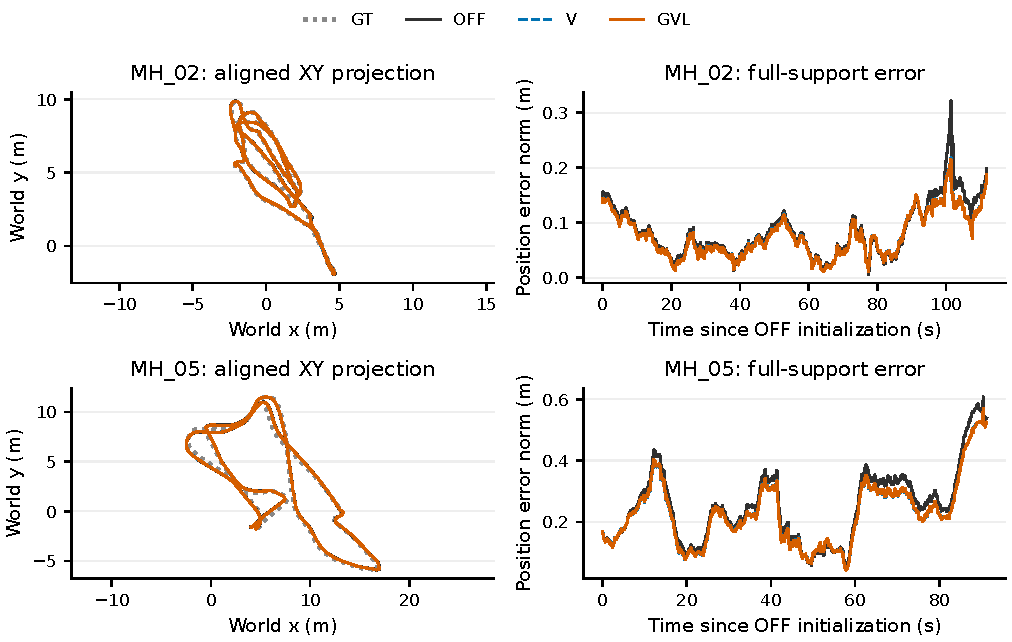
\includegraphics[width=\textwidth]{figures/trajectory_errors.pdf}
\caption{Archived MH\_02 and MH\_05 trajectories and position errors for OFF, V, and GVL. Left: XY projections after full-support rigid alignment without scale. Right: unsmoothed three-dimensional position-error norms, using the identical OFF-matched timestamps. Each mode uses one alignment over the full matched trajectory.}
\label{fig:trajectory_errors}
\end{figure*}

\subsection{Relative Motion and Local Error}
Table~\ref{tab:mhmetrics} examines whether the ATE improvements are accompanied by changes in relative motion and error extremes. GVL lowers 1 s and 5 s translation RPE, final-support position RMSE, and maximum position error on all four evaluated MH sequences. On MH\_02, the final-support RMSE reduction is 21.48\%, and the maximum aligned position error reduction is 33.01\%. These measurements provide complementary evidence to full-trajectory ATE.
\begin{table}[tb]
\caption{Relative error reductions of GVL against OFF in Machine Hall (\%). Tail is position RMSE over the final 10\% of matched support; max is the maximum aligned position error.}\label{tab:mhmetrics}
\centering\small
\begin{adjustbox}{max width=\columnwidth}
\begin{tabular}{lrrrrr}
\toprule
Sequence & ATE & RPE-T 1 s & RPE-T 5 s & Tail & Max \\
\midrule
MH\_01 & 1.44 & 4.61 & 1.83 & 2.85 & 0.30 \\
MH\_02 & 11.54 & 8.88 & 5.92 & 21.48 & 33.01 \\
MH\_03 & 8.85 & 2.31 & 2.43 & 11.07 & 6.95 \\
MH\_05 & 8.49 & 2.31 & 1.47 & 8.48 & 6.34 \\
\bottomrule
\end{tabular}
\end{adjustbox}
\end{table}

Overall improvements do not imply that every local interval improves. In the fixed 10 s analysis, the largest relative GVL increase is 9.018\% (3.368 mm) in MH\_03 window index 5. V increases the same window by 8.552\% (3.193 mm). The largest absolute GVL window increase is about 5.821 mm in V2\_03 window index 11. G has a maximum relative local increase of 6.081\% (2.754 mm) in MH\_01 window index 7. These outcomes are reported alongside the gains rather than hidden by a trajectory-level average.
Figure~\ref{fig:local_windows} displays all archived windows for these two sequences, including the local increases.
\begin{figure*}[t]
\centering
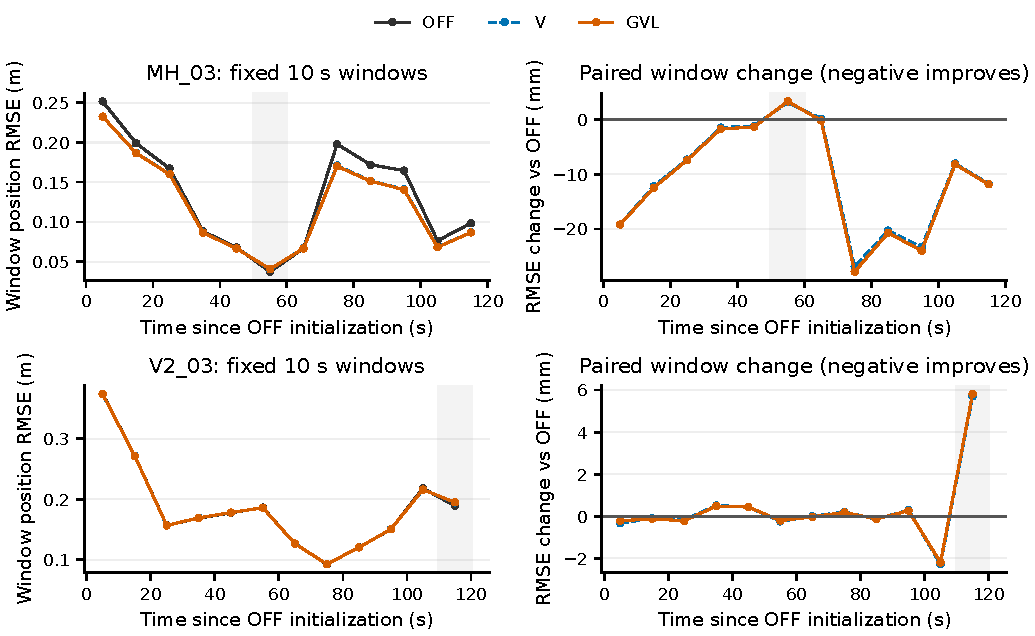
\includegraphics[width=\textwidth]{figures/local_window_errors.pdf}
\caption{Fixed 10 s window errors in MH\_03 and V2\_03. Left: absolute position RMSE. Right: paired changes relative to OFF in millimetres; negative values indicate improvement. Shading marks window indices 5 and 11, respectively. Windows retain the full-trajectory alignment and baseline support; the final window may have partial support.}
\label{fig:local_windows}
\end{figure*}

\subsection{Actual Auxiliary Use and Computational Cost}
Table~\ref{tab:updates} reports the frames in which each GVL branch was actually applied. Nonzero application counts on every evaluated sequence distinguish active fusion from merely enabling a configuration flag. Different counts are expected because landmark maturity, live anchors, and gravity/velocity readiness are separate checks.
\begin{table}[tb]
\caption{Frames with actually applied auxiliary branches in GVL. Counts can differ because each branch has its own validity conditions.}\label{tab:updates}
\centering\small
\begin{adjustbox}{max width=\columnwidth}
\begin{tabular}{lrrr}
\toprule
Sequence & G & V & L \\
\midrule
MH\_01 & 2350 & 2343 & 2343 \\
MH\_02 & 1499 & 1478 & 1478 \\
MH\_03 & 2078 & 1929 & 1927 \\
MH\_05 & 1638 & 1578 & 1578 \\
V1\_01 & 2426 & 2407 & 2406 \\
V1\_02 & 953 & 932 & 930 \\
V1\_03 & 956 & 931 & 927 \\
V2\_01 & 1574 & 1563 & 1560 \\
V2\_02 & 1606 & 1571 & 1570 \\
V2\_03 & 706 & 637 & 627 \\
\bottomrule
\end{tabular}
\end{adjustbox}
\end{table}

Resource measurements use complete serial input replays, an exclusive performance lock, the same two-logical-CPU affinity, a verified single OpenCV thread, and the same diagnostic level. Mode order alternates forward and reverse by sequence. The table aggregates paired increases by first computing each sequence's percentage change against OFF and then taking the median.
\begin{table}[tb]
\caption{Median per-sequence increases over OFF (\%). Camera P95 measures only the camera API; full-run CPU and wall time include the complete replay. One serial paired measurement per sequence and mode.}\label{tab:cost}
\centering\small
\begin{adjustbox}{max width=\columnwidth}
\begin{tabular}{lrrrr}
\toprule
Mode & Camera P95 & CPU time & Wall time & Peak RSS \\
\midrule
G & +337.14 & +214.81 & +214.88 & +22.94 \\
V & +335.27 & +214.46 & +214.61 & +22.74 \\
L & +341.14 & +218.42 & +218.65 & +22.92 \\
GVL & +340.78 & +219.22 & +219.40 & +21.69 \\
\bottomrule
\end{tabular}
\end{adjustbox}
\end{table}

Figure~\ref{fig:runtime_cost} shows the sequence-level paired ratios underlying the cost summary.
\begin{figure*}[t]
\centering
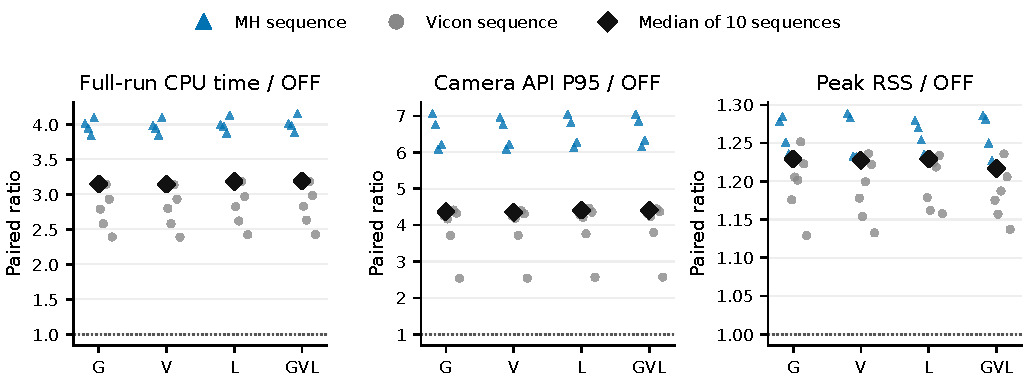
\includegraphics[width=\textwidth]{figures/runtime_cost.pdf}
\caption{Archived serial resource costs relative to OFF for the same sequence. Triangles and circles are the four MH and six Vicon sequence pairs, respectively; diamonds are their medians. A ratio of one denotes the OFF cost. Horizontal offsets only separate categorical points. Each pair has one serial measurement, so the spread describes variation across sequences, not timing confidence intervals.}
\label{fig:runtime_cost}
\end{figure*}

GVL increases median full-run CPU time by 219.22\%, corresponding to approximately 3.19 times the OFF CPU time. Its camera API P95 increases by 340.78\%, while peak resident memory increases by 21.69\%. The absolute GVL camera P95 values range from about 27.07 to 44.68 ms in this measured environment. The camera API does not include the complete IMU and input/output processing path; full-run measurements are therefore reported separately.

Only one paired serial measurement is available for each sequence and mode, so these timings are descriptive measurements without independent timing confidence intervals. The measured ON camera P95 and peak-memory increases exceed the archive's historical 5\% and 10\% overhead limits in every pair. These outcomes concern computational cost and do not invalidate the separately measured trajectory improvements.

\subsection{Discussion}
The archived comparison identifies an operating regime in which the velocity-aided configuration improves Machine Hall trajectories, while the Vicon profiles produce nearly the same full-trajectory position ATE. Both categories are reported because an overall mean hides their different responses; scene-dependent weights also prevent attributing this difference solely to scene geometry. They also motivate evaluating a fixed parameter-selection rule on sequences not used for tuning in future work.

The modest additional benefit of G/L means that enabling every branch should be justified by the application and its error metrics. The landmark branch participates in many updates, yet its standalone ATE benefit is small; application count is evidence of execution, not a guarantee of benefit. Moreover, the mode-dependent weights mean that these results do not isolate all pairwise interactions among the three branches.

The archived implementation measurements show a substantial resource cost. Similar measured costs across G, V, L, and GVL suggest that profiling the common observer and integration path is a useful next step, although the present measurements do not attribute runtime to individual internal operations. The method should consequently be evaluated as an accuracy--cost trade-off rather than presented as a lightweight enhancement.

\subsection{Evidence Limits and Further Experimental Validation}
The completed evaluation controls native settings, sensor input, trajectory support, and resource-measurement conditions across modes. It is a tuned configuration comparison: a strict branch ablation would keep the same enabled-branch weights in single and combined modes and change only the branch switches. The present archive does not contain such an ablation or a held-out dataset evaluation. These are further experimental requirements, not completed results.

A follow-up protocol should freeze weights using only a declared development set, then evaluate them unchanged on sequences or a dataset not used for tuning. All selected sequences, including initialization or tracking failures, should enter the outcome report; ATE on successful support should be accompanied by initialization delay, output coverage, and failure/recovery counts. MH\_04's prior baseline divergence is an exclusion in the existing archive, and no comparative final-run recovery result is available for it. Local error increases and measured overhead remain part of the current evidence. Repeated serial timings and component profiling should quantify runtime variation and identify the observer, feature-management, and fusion costs.

\section{Conclusion}
This paper describes an engineering integration of a body-frame LTV observer with a native visual-inertial filter. The continuous observer supplies the design background, while the discrete algorithm specifies IMU propagation, Joseph bearing correction, bounded landmark initialization and management, and pre/post-camera snapshot timing. G/V/L auxiliary models use matched FEJ Jacobians, validity gates, and noise-based fusion control, and are combined with native visual constraints in one common-prior EKF update under an explicit correlation approximation.

The archived EuRoC comparison reports lower ATE for V and GVL on all four evaluated Machine Hall sequences, with mean relative reductions of 7.410\% and 7.578\%. Vicon position ATE changes are small, some local windows deteriorate, and measured runtime overhead is substantial. These results support a scene- and configuration-dependent accuracy--cost assessment. Strict common-weight ablation, held-out evaluation, complete failure reporting, and repeated runtime profiling remain the next steps for strengthening the empirical conclusions.

\bibliographystyle{splncs04}
\bibliography{references}
\end{document}
